\subsection{Data Overview}
Three different datasets were acquired for this project. Jane Hendry, UCT's CIO, provided data on first-time undergraduates including demographic information, matric results, and admission-acceptance test results (the \textit{FU} dataset). Stephen Marquard, the Learning Technologies Coordinator from the Center for Innovation in Learning and Teaching at UCT (the CILT) provided Sakai \textit{grade} and \textit{event} data. All three of these datasets include a student ID field, which was anonymized by Associate Professor Sonia Berman and, in the case of the \textit{event} data, Stephen Marquard. The anonymized student ID number field is anonymized consistently across all three datasets, making these datasets relatable and suitable for joining.

\textit{Event} data was received for the 2016 academic year and comprises approximately 43 million rows of Sakai events of different 'event types'. This project considered only \textit{events} of type \textit{presence}, identified via an \textit{event\_id} of the value \textit{281}. This translates to roughly 13 million applicable events (i.e. rows). The data model of Sakai events is actually more complicated than the the CSV export shows - the CSV is the output of a SQL \textit{View}, which selects from a subset of tables. The entity-event model prior receiving the CSV export is shown in \ref{SakaiEventModel}.

\begin{figure}[h]
    \centering
    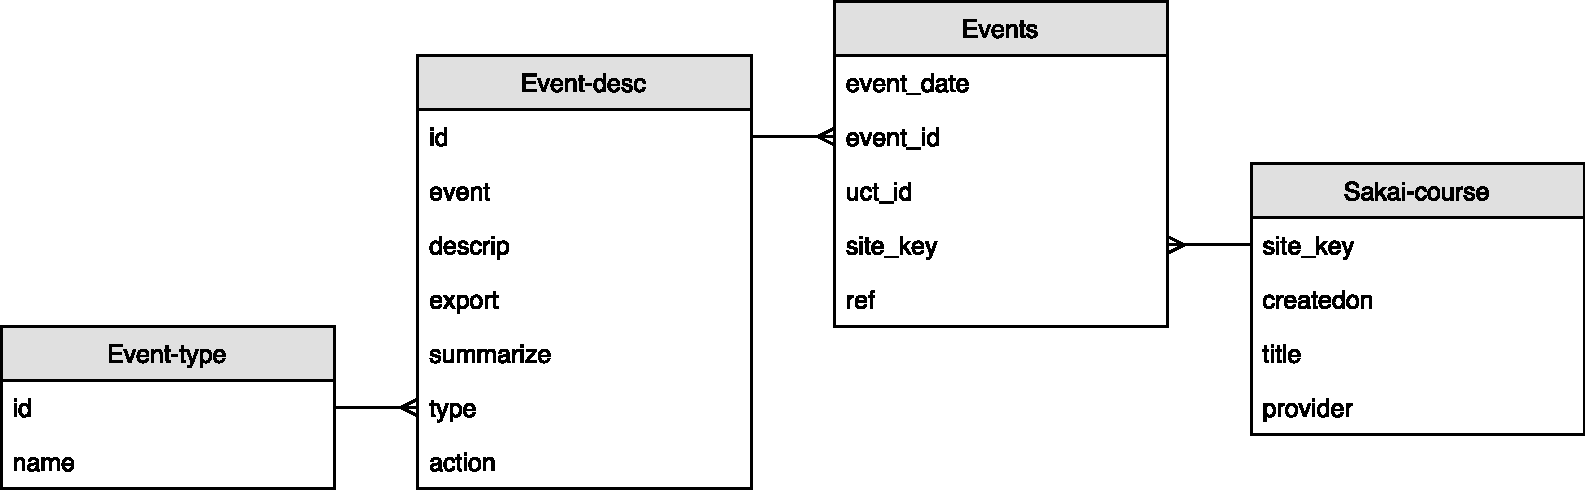
\includegraphics[scale=0.4]{./resources/figures/SakaiEvents}
    \caption[SakaiEventModel]{SakaiEventModel}
    \label{SakaiEventModel}
\end{figure}

\textit{Course grade} data was received for 2014, 2015, and 2016. The field \textit{course\_id} was found to not correspond with the \textit{event} data field \textit{site\_key}, meaning that the \textit{event} and \textit{grade} data is only relatable by year and student ID, and not per individual course.

Demographic data (the \textit{FU} dataset) was includes the years 2014, 2015 and 2016. The schema of this dataset is not consistent across the different years, since in addition the registrant data, a row includes a summary of academic performance at UCT for subsequent years. As a result there were many repeated fields in these datasets and required manual processing before they were of use. Rows from all years of the demographic data were combined into a single sheet with a common list of fields as shown in \ref{appendix:data}. The grade data from all three years was also combined into a single sheet in Excel (without altering any field names of any entities) since a single CSV source for a single data entity is easier to handle in \textit{nETL} and can be processed under a single task instead of 3 separate tasks. For a description of the three data entities provided by UCT refer to the appendix (\ref{appendix:data}), where a description of each field is shown and notes about how each field is treated is shown.

Also in appendix \ref{appendix:data} is an example of each entity represented as JSON and as used by CouchDB. Filtering as mentioned on tables (\ref{event-data-csv}, \ref{grade-data-csv}, \ref{demographic-data-csv}) was performed in the \textit{nETL} application, specified as a \textit{transformation}. The module is shown in the appendix at \ref{netl-trans-filter}. In addition to filtering, an attribute was added to each row imported from the CSVs: \textit{\_type} - so that each document can be identified as a conceptual member of a particular entity. This additional attribute was appended to each row also via the \textit{nETL} application; code to show how such a \textit{transformation} is achieved is included in \ref{netl-trans-create-obj-field}.

For the grade data, further filtering is required on the \textit{RegCareer} field as shown in \ref{appendix:data} and on course suffixes as shown in \ref{appendix:data}. In addition, certain values of the \textit{Percent} attribute need to be scrubbed to normalize these values as numbers - a description of the logic used for this is shown in \ref{appendix:data}. Similarly to the event entity as mentioned above, an attribute has been added to each CSV row to identify the Course Grade entity within CouchDB. A resultant course grade in CouchDB looks like this:

Preprocessing in this project was aimed at reducing the number of dependent variables that are included in the dataset used for analysis (housed in CouchDB). The result is looking at undergraduate course results for South African students over the normal academic year (either 1st semester, 2nd semester or whole year courses).